\documentclass[reqno]{amsart}

\usepackage{external/takodachi}
\renewcommand{\emph}{\textsc}

% Title: change problem set number as needed
\title
{
	\emph{Multi-linear algebra}
} 

\author{Jason Zhao}
\date{\today}

\begin{document}
\maketitle

\begin{abstract}
	These notes serve as a short primer for multi-linear algebra with a view towards geometry. We use \cite[Chapter 12]{Lee2012} as a reference. 
\end{abstract}	

\tableofcontents

\section{Change of basis}
Before getting into any multi-linear algebra, it is important to get a grasp of coordinates in linear algebra and how these coordinates respond to change of bases. Let $V$ be an $n$-dimensional real vector space, and denote $V^*$ its dual space. Given a basis $\{e_i\}_i \subseteq V$, there exists a dual basis $\{\epsilon^j\}_j \subseteq V^*$ satisfying 
	\[ \langle e_i, \epsilon^j \rangle = \delta^j_i. \]
Choose another basis $\{\widetilde e_i\}_i \subseteq V$ and denote its dual basis by $\{\widetilde \epsilon^j\}_j \subseteq V^*$. There exists a change of basis matrix $C^k_i \in \mathsf{GL} (\R^n)$ sending the original basis to the new basis,
	\[ \widetilde e_i = C^k_i e_k. \]	
On the other hand, the inverse change of basis matrix $(C^{-1})^j_k \in \mathsf{GL} (\R^n)$, i.e. $(C^{-1})^j_k C^k_i = \delta^j_i$, transforms the original dual basis to the new dual basis 	
	\[ \widetilde \epsilon^j = (C^{-1})^j_k \epsilon^k. \]
Throughout these notes, we will use these \emph{Einstein summation notation}, where repeated indices are summed over, e.g. $a^i b_i := \sum_i a^i b_i$.


\subsection{{Contravariance}}

We say an object is \emph{contravariant} if the coordinate representation \textit{contra-varies} with respect to change of basis, that is, transforms by the inverse matrix $(C^{-1})^j_i$. Such coordinates are indexed by \textit{upper indices}. The prototypical example of a contravariant object is a \emph{vector} $v \in V$. Every vector admits a unique coordinate representation $\{v^i\}_i \subseteq \R$ with respect to the basis $\{e_i\}_i$, i.e.
	\[ v = v^i e_i . \]
Let $\{ \widetilde v^j \}_j \subseteq \R$ be the unique coordinates with respect to the basis $\{\widetilde e_j\}_j$, then the change of coordinates from $\{v^i\}_i$ to $\{\widetilde v^j\}_j$ is given by the inverse change of basis matrix,
	\[ \widetilde v^j = {(C^{-1})}^j_i v^i. \]
Indeed, 	
	\[ v = \widetilde v^j \widetilde e_j  = \left( {(C^{-1})}^j_i v^i \right) \left( C^k_j e_k \right) = \delta^k_i v^i e_k = v^i e_i . \]
We can interpret a choice of basis $\{e_i\}_i$ as endowing $V$ with a ``measuring tool'', where the coordinates $\{v^i\}_i$ representing the resulting ``measurement''. A change of basis corresponds to changing the choice of ``measuring tool'', e.g. we can view a change of basis $\widetilde e_i = \tfrac{1}{100} e_i$ as changing from ``meters'' $e_i$ to ``centimeters'' $\widetilde e_i$, so the corresponding change of coordinates is 
	\[ \widetilde v^i \text{ meters } = 100 v^i \text{ centimeters}. \]




\subsection{Covariance}

We say that an object is \emph{covariant} if the coordinate representation \textit{co-varies} with respect to change of basis, that is, transforms by the matrix $C^k_i$.  Such coordinates are indexed by \textit{lower indices}. The prototypical example of a covariant object is a \emph{covector} $\omega \in V^*$. Every covector admits a unique coordinate representation $\{\omega_i \}_i \subseteq \R$ with respect to the basis $\{\epsilon^i\}_i$, i.e.
	\[ \omega = \omega_i \epsilon^i = \widetilde \omega_j \widetilde \epsilon^j. \]
Let $\{\widetilde \omega_j \}_j \subseteq \R$ be the unique coordinates with respect to the basis $\{\widetilde \epsilon^j\}_j$, then the change of coordinates from $\{\omega_i\}_i$ to $\{\widetilde \omega_j\}_j$ is given by the change of basis matrix,
	\[ \widetilde \omega_j = C^i_j \omega_i \]
Indeed, 
	\[ \omega = \widetilde \omega_j \widetilde \epsilon^j = \left( C^i_j \omega_i \right) \left( (C^{-1})_k^j \epsilon^k \right) =  \delta^i_k \omega_i \epsilon^k = \omega_i \epsilon^i. \]
Scalars are regarded as ``dimensionless'' quantities, so since a covector acting on a vector produces a scalar, they have inverse dimensions. For example, we can view a change of basis $\widetilde \epsilon^j = 100 \epsilon^j$ as changing from  ``meters$^{-1}$'' $\epsilon^j$ to ``centimeters$^{-1}$'' $\widetilde \epsilon^j$, so the corresponding change of coordinates is 
	\[ \widetilde \omega_j \text{ meters$^{-1}$} = \frac{1}{100} \omega_j  \text{ centimeters$^{-1}$}. \]



\section{Tensors}
A tensor is an object which encodes information about a multi-linear relationship between vectors and co-vectors. We present three equivalent definitions which are well-suited for their respective contexts. 



\subsection{Multi-linear functionals}

The simplest and most intuitive definition of a tensor is that it is a multi-linear functional, i.e. a functional which is linear in each of its arguments. A \emph{$(k, \ell)$-tensor} is a $(k + \ell)$-linear functional
	\[ \overbrace{V^* \times \dots \times V^*}^{\text{$k$-copies}} \times \overbrace{V \times \dots \times V}^{\text{$\ell$-copies}}  \to \R. \]
We denote the \emph{space of $(k, \ell)$-tensors} by $T^{(k, \ell)} (V)$, where by convention $T^{(0, 0)} (V) := \R$. More precisely, this is the space of tensors which are $k$-contravariant and $\ell$-covariant. 

\begin{example}
\leavevmode
\begin{enumerate}
	\item A vector, using the natural identification with the double dual space, $v\in V$ is a $(1, 0)$-tensor, while a co-vector $\omega \in V^{*}$ is a $(0, 1)$-tensor. 
	
	\item An inner product $ g: V \times V \to \R$ is a symmetric $(0, 2)$-tensor. 
	
	\item A linear transformation $T : V \to V$ can be identified with the $(1, 1)$-tensor given by 
			\[ (\omega, v) \mapsto \langle T(v), \omega \rangle.\]
		More generally, if $T: (V^*)^k \times V^\ell \to V$ is multi-linear, then it can be identified with the $(k + 1, \ell)$-tensor
			\[ (\omega_1, \dots, \omega_k, \omega_{k + 1}, v_1, \dots, v_\ell) \mapsto \langle T(\omega_1, \dots, \omega_k, v_1, \dots, v_\ell) , \omega_{k + 1}\rangle .\]
		
	
	\item In view of (c), the cross product $\times : \R^3 \times \R^3 \to \R^3$ is a $(1, 2)$-tensor. 

\end{enumerate}
\end{example}


\subsection{Coordinate representations}

When performing computations with tensors, it is convenient to work with the coordinate representations. These coordinates are defined with respect to a natural choice of basis for the space of tensors. Abbreviating the multi-indices $I:= (i_1, \dots, i_k)$ and $J := (j_1 ,\dots j_\ell)$, the collection of tensors $\{ e_{i_1} \otimes \dots \otimes e_{i_k} \otimes \epsilon^{j_1} \otimes \dots \otimes \epsilon^{j_\ell} \}_{I, J} \subseteq T^{(k, \ell)} (V)$ forms a basis. More precisely, each $T \in T^{(k, \ell)} (V)$ admits the unique \emph{coordinate representation}
		\begin{align*}
			T 
				&= T^{i_1\dots i_k}_{j_1 \dots j_\ell} e_{i_1} \otimes \dots \otimes e_{i_k} \otimes \epsilon^{j_1} \otimes \dots \otimes \epsilon^{j_\ell} ,
		\end{align*}
	with coordinates given by $T^{i_1\dots i_k}_{j_1 \dots j_\ell} := T(\epsilon_{i_1}, \dots , \epsilon_{i_k} ,e^{j_1} , \dots, e^{j_\ell})$. This also shows that $\dim T^{(k, \ell)} (V) = (\dim V)^{k + \ell}$. This can be checked by evaluating $T$ and its coordinate representation on $k$-tuples of co-vectors $\omega = \omega_i \epsilon^i$ and $\ell$-tuples of vectors $v = v^i e_i$, computing each appropriately to show that they agree, and that the coefficients vanish $ T^{i_1\dots i_k}_{j_1 \dots j_\ell} = 0$ if and only if $T \equiv 0$. These coordinates obey the \emph{transformation law}
		\[ \widetilde T^{i_1'\dots i_k'}_{j_1' \dots j_\ell'} = (C^{-1})^{i_1'}_{i_1} \cdots  (C^{-1})^{i_k'}_{i_k} T^{i_1\dots i_k}_{j_1\dots j_\ell} C^{j_1}_{j_1'} \cdots C^{j_\ell}_{j_\ell'}, \]
	where $\{ \widetilde T^{i_1'\dots i_k'}_{j_1' \dots j_\ell'} \}_{I, J} \subseteq \R$ denote the unique coordinates with respect to the basis $\{\widetilde e_j\}_j$. That is, the upper indices transform contravariantly, i.e. with respect to the inverse change of basis matrix, and the lower indices transform covariantly, i.e. with respect to the change of basis matrix. We sometimes indent the indices if the order of the arguments is important, e.g. if $T: V \times V^* \times V \to \R$ is multi-linear, then 
		\[ T = T\indices{_\alpha^\beta_\gamma} \epsilon^\alpha \otimes e_\beta \otimes \epsilon^\gamma. \] 

\begin{example}
\leavevmode
\begin{enumerate}
	\item Vectors and co-vectors have coordinate representations $v = v^i e_i$ and $\omega = \omega^j \epsilon_j$, where the coordinates can be computed by testing against the dual basis $v^i := \langle v, \epsilon^i \rangle$ and $\omega_j := \langle e_j, \omega \rangle$. 
	
	
	\item If $\{e_i\}_i \subseteq V$ is an orthonormal basis with respect to the inner product $g : V \times V \to \R$, then $g = \delta^{ij} \epsilon_i \otimes \epsilon_j$.
	
	\item We can write the image of the basis under a linear transformation $T: V \to V$ as $Te_i = T^j_i e_j$. The coefficients $T^j_i$ are precisely those when $T$ is viewed as a $(1, 1)$-tensor in this basis. 
	
	\item Let $\{e_1, e_2, e_3\} \subseteq \R^3$ be the standard Euclidean basis, then the cross product is $v \times w = \epsilon\indices{^i_j_k}  e_i v^j w^k$.
	
\end{enumerate}
\end{example}
	
\begin{remark}
	In view of the existence and uniqueness of coordinates, we can alternatively characterise a tensor as a map sending a basis for $V$ to a $(k + \ell)$-dimensional array of coordinates satisfying the transformation law. Denote $\operatorname{Fr} (V)$ the space of ordered bases on $V$, there is a natural action by the general linear group $\mathsf{GL} (\R^n)$. Let $\rho : \mathsf{GL} (\R^n) \to \mathsf{GL} (\R^{n^{k + \ell}})$ be the group homomorphism 
		\[ 
			\rho(C) 
				:=
				\operatorname{diag} (\overbrace{C^{-1}, \dots, C^{-1}}^{k\text{-times}}, \overbrace{C, \dots, C}^{\ell\text{-times}}).
		\]
	Then a $(k, \ell)$-tensor is a map $T: \operatorname{Fr} (V) \to \R^{n^{k + \ell}}$ which is $\rho$-equivariant, 
		\[ T(C \beta) = \rho(C) T(\beta). \]
	This is the perspective of \textit{representation theory}; we will not need this level of abstract nonsense. 
	
	\end{remark}	
	
\subsection{Tensor products of vector spaces}

In linear algebra, a vector is defined as an element of a vector space. Analogously, we can take an intrinsic approach to tensors, viewing them as elements of an algebraic construction. For notational convenience, we work in full generality: let $V_1, \cdots, V_k$ be real vector spaces, the \emph{free vector space} $F(V_1 \times \dots \times V_k)$ is the set of all formal linear combinations of symbols $(v_1, \dots, v_k) \in V_1 \times \dots \times V_k$. Let $R(V_1 \times \dots \times V_k) \hookrightarrow F(V_1 \times \dots \times V_k)$ be the subspace generated by the $k$-linear relations
	\[		(v_1, \dots, av_i, \dots, v_k) - a(v_1, \dots, v_i, \dots, v_k), \]
	\[	
		(v_1, \dots, v_i + w_i, \dots, v_k) - (v_1, \dots, v_i, \dots, v_k) - (v_1, \dots, w_i, \dots, v_k)
	\]
for $v_j, w_j \in V_j$ and $a \in \R$ and $i = 1, \dots, k$. The \emph{tensor product} of $V_1, \dots, V_k$ is defined as the quotient 
	\[ V_1 \otimes \dots \otimes V_k := F(V_1 \times \dots \times V_k) / R(V_1 \times \dots \times V_k).\]


\begin{lemma}[Universal property of tensor products]
	Let $V_1, \dots, V_k$ and $U$ be finite dimensional vector spaces and denote by $\iota : V_1 \times \dots \times V_k \to V_1 \otimes \dots \otimes V_k$ the $k$-linear map $(v_1, \dots, v_k) \mapsto v_1 \otimes \dots \otimes v_k$. Then for every $k$-linear map $\phi : V_1 \times \dots \times V_k \to U$, there exists a unique linear map $\widetilde \phi :  V_1 \otimes \dots \otimes V_k  \to U$ such that the diagram commutes
	\begin{center}
		\begin{tikzcd}
V_1 \times \dots \times V_k \arrow[r, "\iota"] \arrow[rd, "\phi"'] &  V_1 \otimes \dots \otimes V_k  \arrow[d, "\widetilde \phi"] \\
                                           & U                                         
\end{tikzcd}
	\end{center}
\end{lemma}

\begin{proof}
	By the universal property of free vector spaces, there exists a unique linear map $\overline \phi : F(V_1 \times \dots V_k) \to U$ induced by 
		\[ \overline \phi (v_1, \dots, v_k) := \phi(v_1, \dots, v_k).  \]
	We see from $k$-linearity of $\phi$ that $R(V_1 \times \dots \times V_k) \hookrightarrow \ker \overline \phi$, so $\overline \phi$ descends to $\widetilde \phi : V_1 \otimes \dots \otimes V_k \to U$ the unique linear map satisfying 
		\[ \widetilde \phi (v_1 \otimes \dots \otimes v_k) = \overline \phi (v_1, \dots, v_k) = \phi(v_1, \dots, v_k). \]
	The condition above can be rewritten as $\widetilde \phi \circ \iota = \phi$, completing the proof. 
\end{proof}

\begin{theorem}[Equivalence of definitions]
	Let $V$ be a finite dimensional vector space, then there is a canonical isomorphism
		\[ {V}^{\otimes k} \otimes {(V^*)}^{\otimes \ell} \cong T^{(k, \ell)} (V).  \]
\end{theorem}

\begin{proof}
	Each tensor $T \in T^{(k, \ell)} (V)$ is a mult-linear map $T: (V^*)^k \times V^\ell  \to \R$, so by the universal property there exists unique corresponding linear map $\widetilde T : {(V^*)}^{\otimes k} \otimes {V}^{\otimes \ell} \to \R$, which we can view as an element of the dual space $\widetilde T \in ({(V^*)}^{\otimes k} \otimes {V}^{\otimes \ell})^*$. It is easy to check that the map $T \mapsto \widetilde T$ is linear, and furthermore by the universal property we can construct a natural isomorphism between the dual of tensor products and the tensor products of dual spaces, $({(V^*)}^{\otimes k} \otimes {V}^{\otimes \ell})^* \cong {V}^{\otimes k} \otimes {(V^*)}^{\otimes \ell}$. This completes the proof. 
\end{proof}




\section{Symmetric and alternating tensors}

\subsection{Symmetrisation}

Let $S_k$ denote the \emph{symmetric group}, the set of permutations of the set $\{1, \dots, k\}$. There is a natural action on the space of $k$-tuples $V^k$; we say that a covariant $k$-tensor $T \in T^k (V^*)$ is \emph{symmetric} if $T$ is invariant with respect to this action, i.e.
	\[ T(v_1, \dots, v_k) = T(v_{\sigma(1)}, \dots, v_{\sigma(k)}) \]
for all permutations $\sigma \in S_k$. In particular, given a basis $\{v_i\}_i$, we see that $T$ is symmetric if and only if its coordinates are symmetric in its indices, 
	\[ T_{i_1 \dots i_k} = T_{\sigma(i_1) \dots \sigma(i_k)}. \]
Denote the space of symmetric tensors by $\Sigma^k (V^*)$, there is a projection $\operatorname{Sym} : T^k (V^*) \to \Sigma^k (V^*)$ known as the \emph{symmetrisation},
	\[ \operatorname{Sym} T (v_1, \dots, v_k) := \frac{1}{k !} \sum_{\sigma \in S_k} T(v_{\sigma(1)}, \dots, v_{\sigma(k)}). \]
It is easy to check that symmetrisation acts identically on symmetric tensors. 

\begin{example}
	Inner products are the prototypical example of symmetric tensors. 
\end{example}

\subsection{Alternation}

We say that the tensor $T \in T^k (V^*)$ is \emph{alternating} if it is invariant under action by the symmetric group up to the sign of the permutation 
	\[ T(v_1, \dots, v_k) = (-1)^\sigma T(v_{\sigma(1)}, \dots, v_{\sigma(k)}) \]
for all permutations $\sigma \in S_k$. In particular, given a basis $\{v_i\}_i$, we see that $T$ is alternating if and only if its coordinates are anti-symmetric in its indices, 
	\[ T_{i_1 \dots i_k} = (-1)^\sigma T_{\sigma(i_1) \dots \sigma(i_k)}. \]
Denote the space of alternating tensors by $\Lambda^k (V^*)$, there is a projection $\operatorname{Alt} : T^\ell (V^*) \to \Lambda^k (V^*)$ known as the \emph{alternation},
	\[ \operatorname{Alt} T (v_1, \dots, v_k) := \frac{1}{k !} \sum_{\sigma \in S_k} (-1)^\sigma T(v_{\sigma(1)}, \dots, v_{\sigma(k)}). \]
It is easy to check that alternation acts identically on alternating tensors. 

\begin{remark}
	The following are equivalent:
	\begin{enumerate}
		\item $T$ is alternating, 
		\item $T(v_1, \dots, v_k) =0$ whenever $(v_1, \dots, v_k)$ is linearly dependent, 
		\item $T$ vanishes whenever two of its arguments are equal, $T(v_1, \dots, w, \dots, w, \dots, v_k) = 0$. 
	\end{enumerate}
\end{remark}

\begin{example}
	The prototypical example of an alternating tensor is the determinant. 
\end{example}


\section{Tensor algebra}
Taking the direct sum of $T^{(k, \ell)} (V)$ for every $k, \ell \geq 0$, we can form a vector space which is \textit{graded} by the rank of the tensors $(k, \ell)$. In this section we will define two operations which move tensors from one grade to another grade, the first of which, the tensor product $\otimes : T(V) \times T(V) \to T(V)$, endows the \emph{tensor algebra}
	\[ T(V) := \bigoplus_{k, \ell} T^{(k, \ell)} (V) \]
with the structure of an \textit{associative graded algebra}. 	

\subsection{Products}

Define the \emph{tensor product} $\otimes : T^{(k, \ell)}(V) \times T^{(p, q)}(V) \to T^{(k + p, \ell + q)}(V)$ defined by 
	\[ (S \otimes T) (\omega^1, \dots, \omega^{k + p}, v_1, \dots, v_{\ell + q}) = S(\omega^1, \dots, \omega^k, v_1, \dots, v_\ell) T(\omega^{k + 1}, \dots, \omega^{k + p}, v_{\ell + 1}, \dots, v_{\ell + q}). \]
The operation in coordinates amounts to pairwise multiplication, i.e.
	\[ (S \otimes T)^{i_1 \dots i_k i_{k + 1} \dots i_{k + p}}_{j_1 \dots j_\ell j_{\ell + 1} \dots j_{\ell + q}} = S^{i_1 \dots i_k}_{j_1 \dots j_\ell} T^{i_{k + 1} \dots i_{k + p}}_{j_{\ell + 1} \dots j_{\ell + q}}. \]
Using the tensor product, we can construct a natural basis for $T^{(k, \ell)} (V)$ provided a basis for $V$: 	

\begin{proposition}[Basis for $T^{(k, p)} (V)$]
	Let $\{ e_i \}_i \subseteq V$ and $\{ \epsilon^j\}_j \subseteq V^*$ form dual bases, then 
		\[ \{ e_{i_1} \otimes \dots \otimes e_{i_k} \otimes \epsilon^{j_1} \otimes \dots \otimes \epsilon^{j_\ell} \}_{I, J} \subseteq T^{(k, \ell)} (V)\]
	forms a basis. More precisely, each $T \in T^{(k, \ell)} (V)$ admits the unique coordinate representation
		\begin{align*}
			T 
				&= T^{i_1\dots i_k}_{j_1 \dots j_\ell} e_{i_1} \otimes \dots \otimes e_{i_k} \otimes \epsilon^{j_1} \otimes \dots \otimes \epsilon^{j_\ell} ,
		\end{align*}
	with coordinates given by $T^{i_1\dots i_k}_{j_1 \dots j_\ell} := T(\epsilon_{i_1}, \dots , \epsilon_{i_k} ,e^{j_1} , \dots, e^{j_\ell})$. Moreover $\dim T^{(k, \ell)} (V) = (\dim V)^{k + \ell}$.
\end{proposition}

\begin{proof}
	Let $\omega^{(\alpha)} = \omega^{(\alpha)}_j \epsilon^j$ be a collection of co-vectors and $v_{(\beta)} = v^i_{(\beta)} e_i$ a collection of vectors, we use multi-linearity to compute
		\begin{align*}
			T( \omega^{(1)},  \dots, \omega^{(k)}, v_{(1)} , \dots, v_{(\ell)})
				&= T(\epsilon_{i_1}, \dots , \epsilon_{i_k} ,e^{j_1} , \dots, e^{j_\ell})  \omega_{j_1}^{(1)} \dots \omega_{j_k}^{(k)}  v^{i_1}_{(1)} \dots, v^{i_\ell}_{(\ell)} \\
				&=T^{i_1\dots i_k}_{j_1 \dots j_\ell} (e_{i_1} \otimes \dots \otimes e_{i_k} \otimes \epsilon^{j_1} \otimes \dots \otimes \epsilon^{j_\ell}) ( \omega^{(1)},  \dots, \omega^{(k)}, v_{(1)} , \dots, v_{(\ell)}).
		\end{align*}
	This proves the formula. Choosing appropriate combinations of vanishing and non-vanishing coefficients $\omega^{(\alpha)}_j, v^i_{(\beta)} \in \R$ shows that $T^{i_1\dots i_k}_{j_1 \dots j_\ell} = 0$ if and only if $T \equiv 0$, proving uniqueness. 
\end{proof}
	
Using the tensor product and symmetrisation, we can similarly define the \emph{symmetric tensor product} of covariant tensors $\odot : \Sigma^k (V^*) \times \Sigma^p (V^*) \to \Sigma^{k + p} (V^*)$ by  
	\begin{align*}
		(S \odot T)(v_1, \dots, v_k, v_{k + 1}, \dots, v_{k + p}) 
			&:= \operatorname{Sym} (S \otimes T)(v_1, \dots, v_k, v_{k + 1}, \dots, v_{k + p})  \\
			&= \sum_{\sigma \in S_{k + p}} S(v_{\sigma(1)}, \dots, v_{\sigma(k)}) T(v_{\sigma(k + 1)}, \dots, v_{\sigma(k + p)}).
	\end{align*}	
In coordinates, 
	\begin{align*}
		(S \odot T)^{i_1 \dots i_k i_{k + 1} \dots i_{k + p}}_{j_1 \dots j_\ell j_{\ell + 1} \dots j_{\ell + q}} = \sum_{\sigma \in S_{k + p}} S^{i_{\sigma(1)} \dots i_{\sigma(k)}}_{j_{\sigma(1)} \dots j_{\sigma(\ell)}} T^{i_{{\sigma(k + 1)}} \dots i_{{\sigma(k + p)}}}_{j_{{\sigma(\ell + 1)}} \dots j_{{\sigma(\ell + q)}}}.
	\end{align*}	
Since symmetrisation is a projection, it maps a basis to a collection which spans $\Sigma^k (V^*)$. It is clear that the redundancies are precisely $\operatorname{Sym}(e^{i_1} \otimes \cdots \otimes e^{i_k})  = \operatorname{Sym} (\epsilon^{\sigma(i_1)} \otimes \dots \otimes \epsilon^{\sigma(i_k)})$. The collection of $k$-tuples of indices $(i_1, \dots, i_k)$ up to permutation by $S_k$ can be identified with the collection of $k$-tuples satisfying $i_1 \leq \dots \leq i_k$. Thus we have 


	
\begin{proposition}[Basis for $\Sigma^k (V^*)$]
	Let $\{ e_i \}_i \subseteq V$ and $\{ \epsilon^j\}_j \subseteq V^*$ form dual bases, then 
		\[ \left\{ \sum_{\sigma \in S_k} \epsilon^{\sigma(i_1)} \otimes \dots \otimes \epsilon^{\sigma(i_k)}  \right\}_{1 \leq i_1 \leq \dots \leq i_k \leq n} \subseteq \Sigma^k (V^*) \]
	forms a basis. More precisely, each $T \in \Sigma^k (V^*)$ admits the unique coordinate representation
		\[ T = \sum_{1 \leq i_1 \leq \dots \leq i_k \leq n} \frac{1}{\alpha (i_1, \dots, i_k)} T_{{i_1} \dots{i_k}} \sum_{\sigma \in S_k} \epsilon^{\sigma(i_1)} \otimes \dots \otimes \epsilon^{\sigma(i_k)} \]
	where $T_{{i_1} \dots{i_k}} = T(e_{i_1}, \dots, e_{i_k})$ and $\alpha(i_1,\dots,i_k) = m_1! \cdots m_n!$ and $m_j$ is the multiplicity of $j \in \{1, \dots, n\}$ in the tuple $(i_1, \dots, i_k)$. Moreover, $\dim \Sigma^k (V^*) = \binom{n + k - 1}{k}$. 
\end{proposition}

\begin{proof}
	Since $T$ is symmetric, the coordinates are invariant under the symmetric group $ T_{{i_1} \dots{i_k}}  = T_{{\sigma(i_1)} \dots{\sigma(i_k)}}$. Expanding $T$ into coordinates and the implicit sum into a double sum over indices $i_1 \leq \dots \leq i_k$ and $\sigma \in S_k$ \textit{a la} our previous remark, we obtain
	\begin{align*}
		T 
			&=  \sum_{1 \leq i_1 \leq \cdots \leq i_k \leq n} \frac 1{\alpha(i_1,\dots,i_k)} \sum_{\sigma \in S_k} T_{{\sigma(i_1)} \dots{\sigma(i_k)}}  e^{\sigma(i_1)} \otimes \cdots \otimes e^{\sigma(i_k)}\\
			&=  \sum_{1 \leq i_1 \leq \cdots \leq i_k \leq n} \frac 1{\alpha(i_1,\dots,i_k)}  T_{{i_1} \dots{i_k}} \sum_{\sigma \in S_k}  e^{\sigma(i_1)} \otimes \cdots \otimes e^{\sigma(i_k)}.
	\end{align*}
	Uniqueness follows from testing against various $k$-tuples of vectors. 
\end{proof}

\subsection{Trace}	

There is a natural mapping $\operatorname{tr}: V \times V^* \to \R$ known as the \emph{trace} given by pairing the vector and co-vector, 
	\[  (v, \omega) \mapsto \langle v, \omega \rangle, \] 
or, in coordinates, pairing a contravariant index with a covariant index, 
	\[ v^i \omega_j \mapsto v^i \omega_i. \]
Indeed, from the coordinate form, we see that the trace operator coincides with the usual trace operator for matrices when viewing them as $(1, 1)$-tensors. We can generalise the trace operator to a family $\operatorname{tr}^{(p, q)} : T^{(k, \ell)} (V) \to T^{(k - 1, \ell - 1)} (V)$ which takes the trace of the $p$-th contravariant index with the $q$-th covariant index. Tracing a tensor product is sometimes known as \textit{contraction}; more on this later. 




\section{Exterior algebra}


We say that a covariant $k$-tensor  $T: V \times \dots \times V \to \R$ is an \emph{external form} if it is alternating, i.e.
	\[ T(v_1, \dots, v_k) = (-1)^\sigma T(v_{\sigma(1)}, \dots, v_{\sigma(k)}),\]
where $\sigma \in S_k$ is a permutation on the indices $\{1, \dots, k\}$. We denote the space of alternating covariant $k$-tensors by $\bigwedge^k V^*$. The properties of exterior forms axiomatise precisely the expected properties of oriented $k$-volume, namely
\begin{enumerate}
	\item $k$-linearity with respect to the spanning vectors,
	\item degeneracy when two spanning vectors are linearly dependent,
	\item transposition to change orientation.
\end{enumerate}

\begin{figure}[h]
	\begin{center}
		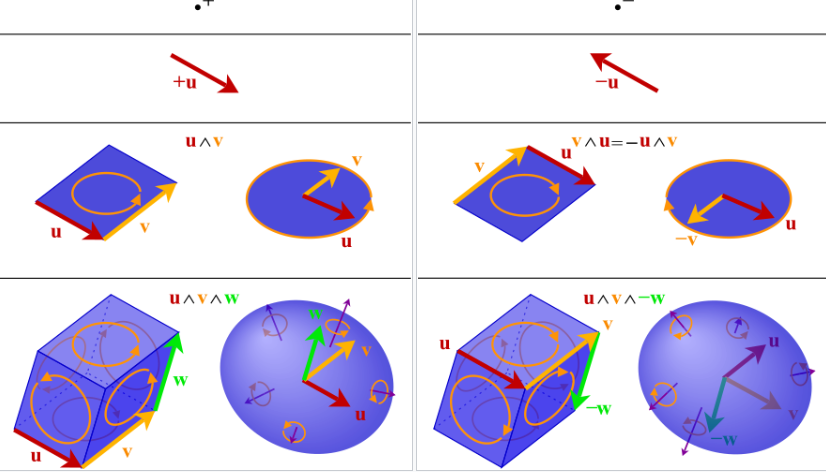
\includegraphics[scale =0.6]{graphics/wedge}
		\caption{Oriented $k$-volume of parallelopiped spanned by an ordered set of $k$-vectors. Changing the order corresponds to changing the orientation.}
	\end{center}
\end{figure}

\subsection{Exterior product}

There exists an associative operation operation known as the \emph{exterior product} $\wedge : \Lambda^k (V^*) \times \Lambda^p (V^*) \to\Lambda^{k + p} (V^*)$ by  
	\begin{align*}
		(S \wedge T) (v_1, \dots, v_k, v_{k + 1}, \dots, v_{k + p}) 
			&:= \frac{(k + p)!}{k! p!}\operatorname{Alt} (S \otimes T)(v_1, \dots, v_k, v_{k + 1}, \dots, v_{k + p})  \\
			&= \frac{1}{k! p!} \sum_{\sigma \in  S_{k + p}} (-1)^\sigma S(v_{\sigma(1)}, \dots, v_{\sigma(k)}) T(v_{\sigma(k + 1)}, \dots, v_{\sigma(k + p)}).
	\end{align*}	
The exterior product is \textit{anti-commutative} in that 
	\[ S \wedge T = (-1)^{k  p} T \wedge S. \]
The choice of coefficient $\tfrac{(k + p)!}{k! p!}$ normalises the exterior product such that it coincides with the determinant. This allows for a clean coordinate representation; compare with the coordinates for symmetric tensors. 
	
\begin{proposition}[Basis for $\bigwedge^k V^*$]
	Let $\{e_i\}_i \subseteq V$ and $\{\epsilon^j\}_j \subseteq V^*$ form dual bases, then 
	\[ \left\{ \epsilon^{i_1} \wedge \dots \wedge \epsilon^{i_k}  \right\}_{1 \leq i_1 < \dots < i_k \leq n} \subseteq\bigwedge^k V^* \]
	forms a basis. More precisely, each $T \in \bigwedge^k V^*$ admits the unique coordinate representation
		\begin{align*}
			T = T_{i_1 \dots i_k} \epsilon^{i_1} \wedge \dots \wedge \epsilon^{i_k},
		\end{align*}
	with coordinates given by $T^{i_1\dots i_k}_{j_1 \dots j_\ell} := T(\epsilon_{i_1}, \dots , \epsilon_{i_k} ,e^{j_1} , \dots, e^{j_\ell})$. Moreover $\dim \bigwedge^k V^* = \binom{n}{k}$ where by convention the binomial coefficient is zero for $k > n$.
\end{proposition}


\begin{example}
	The exterior forms which take the form $v_1 \wedge \dots \wedge v_k$ satisfy
\begin{enumerate}
	\item $k$-linearity of $(v_1, \dots, v_k) \mapsto v_1 \wedge \dots \wedge v_k$,
	\item alternating, $v \wedge v = 0$, 
	\item anti-commutative, $v \wedge w = -  (w \wedge v)$.
\end{enumerate}
The space of $k$-forms $\bigwedge^k V$ are linear combinations of terms of this form. Geometrically, it captures the notion of ``oriented $k$-volume'' of the $k$-parallelopiped spanned by $v_1, \dots, v_k$. 
\end{example}

\subsection{Interior product}

\subsection{Hodge star}




\section{Inner products}
We say that $g: V \times V \to \R$ is an \emph{inner product}, or in geometry a \emph{metric}, on $V$ if it is a positive-definite symmetric $(0, 2)$-tensor. In coordinates, we write
	\[ g = g_{ij} \epsilon^i \otimes \epsilon^j, \]
where $g_{ij}$ is symmetric and positive definite in the sense of matrices. We say that a basis $\{e_i\}_i$ is \emph{orthogonal} with respect to $g$ if the coordinates form a diagonal matrix, and \emph{orthonormal} if $g_{ij} = \delta_{ij}$. By the \textit{Gram-Schmidt algorithm}, we know that an orthonormal basis always exists. 

We can naturally view an inner product as a linear map $g : V \to V^*$ given by 
	\[ v \mapsto g(v, -). \]
In coordinates,
	\[ v^i \mapsto g_{ij} v^i. \]	
It is standard practice to denote $v_i := g_{ij} v^i$, in which case we say that the metric $g$ \textit{lowers an index}. Conversely, since $g$ is non-degenerate, there is an inverse map $g^{-1} : V^* \to V$, where the matrix $(g^{-1})^{ij}$ is simply the inverse matrix of $g_{ij}$. It is known as the \emph{inverse metric tensor}, writing
	\[ g^{-1} = (g^{-1})^{ij} e_i \otimes e_j,  \]
and, viewed as a map from covectors to vectors, 
	\[ \omega \mapsto g^{-1} (\omega, -). \]	
In coordinates, 
	\[ \omega_j \mapsto (g^{-1})^{ij} \omega_j. \]
Again by convention, we denote $\omega^j :=  (g^{-1})^{ij} \omega_j$, in which we say the inverse metric \textit{raises an index}. More generally, we can define a family of operators $g: T^{(k, \ell)} (V) \mapsto T^{(k - 1, \ell + 1)} (V)$ lowering the $p$-th contravariant index and $g^{-1} : T^{(k, \ell)} (V) \mapsto T^{(k + 1, \ell - 1)} (V)$ lowering the $q$-th covariant index. This is sometimes referred to as \textit{metric contraction}, as we can also construct the maps as the tracing the tensor product with the metric. 

\begin{remark}
	From an algebraic point of view, there is no natural isomorphism between $V$ and its dual $V^*$. However, once a specific metric is chosen, we can freely and naturally move between the two; this is known as the \textit{musical isomorphism}. 
\end{remark}

\bibliographystyle{alpha}
\bibliography{external/biblio}
\end{document}